\documentclass[12pt, a4paper]{report}
\usepackage[utf8]{inputenc}
\usepackage[italian]{babel}
\usepackage{float}
\usepackage{graphicx}
\usepackage{newlfont}
\usepackage{hyperref}
\usepackage{multirow}
\usepackage{subfiles}
\usepackage{listings}
\usepackage{multicol}
\usepackage{dsfont}
\usepackage[toc,page]{appendix}
\usepackage{proof}
\usepackage{wrapfig}
\usepackage{amsmath,amssymb,amsthm,textcomp}

\usepackage{listings, xcolor}
\lstset{
tabsize = 1, %% set tab space width
showstringspaces = false, %% prevent space marking in strings, string is defined as the text that is generally printed directly to the console
numbers = left, %% display line numbers on the left
commentstyle = \color{green}, %% set comment color
keywordstyle = \color{blue}, %% set keyword color
stringstyle = \color{red}, %% set string color
rulecolor = \color{black}, %% set frame color to avoid being affected by text color
basicstyle = \small \ttfamily , %% set listing font and size
breaklines = true, %% enable line breaking
numberstyle = \tiny,
}


\title{Report Progetto Compilatori ed Interpreti}
\author{Marco Benito Tomasone 1038815\\
Luca Genova 1038843\\
Simone  Boldrini 1038792}
\date{2021-2022}

\begin{document}
    \maketitle
    \tableofcontents
    \chapter{Introduzione}
    Questo documento è il Report per il progetto del corso di  Compilatori ed Interpreti del prof. Cosimo Laneve A.S. 2021/2022. Il progetto ha come obiettivo quello di costruire un compilatore per il linguaggio \emph{AssetLan}.
    AssetLan è un semplice linguaggio imperativo con asset, in cui i parametri possono  essere sia standard che asset, con ricorsione e senza mutua ricorsione. 
    \section{Grammatica del Linguaggio}
    Ogni programma in AssetLan è formato da quattro parti principali che sono le dichiarazioni di variabili, le dichiarazioni degli asset, le dichiarazioni delle funzioni e la chiamata a delle funzioni. I tipi permessi per le variabili sono  \emph{int} e \emph{bool}, mentre per le funzioni oltre ai due tipi sopracitati è permesso dichiarare funzioni \emph{void}. I parametri asset hanno tipo \emph{asset}. 

    Nella dichiarazione di funzioni oltre al tipo e al nome della funzione bisogna indicare una lista di parametri tra parentesi tonde e una lista di asset tra parentesi quadre. Nel corpo di una funzione è possibile fare molteplici dichiarazioni di variabili e poi definire degli statement. 
    Uno statement può essere un assegnamento, una funzione move che permette di spostare il contenuto di un asset all'interno di un altro asset (svuotando il primo asset), una print, una transfer, una return, un \emph{if-then-else} oppure una chiamata a funzione. 
    Rispetto alla grammatica che ci è stata fornita inizialmente abbiamo apportato due piccole modifiche: 
    \begin{lstlisting}      
function: (type | 'void') ID '('(decp)?')' '['(adec)?']' {' dec* statement* '}' ;
decp: dec;
    \end{lstlisting}  
    La prima è per separare la dichiarazione dei parametri formali di una funzione dalle dichiarazioni delle variabili nel corpo della funzione. Per fare ciò è stato inserito un nuovo simbolo non terminale \emph{decp} che richiama il non terminale \emph{dec}.
    \begin{lstlisting}      
initcall: ID '(' (exp (',' exp)* )? ')' '[' (bexp (',' bexp)* )? ']' ;
bexp: exp  ;
    \end{lstlisting}
La seconda modifica apportata riguarda l'introduzione di un nuovo simbolo \emph{bexp} che sostituisce le chiamate al simbolo exp all'interno dei parametri asset nella chiamata di una funzione. 
    \chapter{Analisi Lessicale e Sintattica}
    Le prime due fasi del compilatore per il linguaggio AssetLan hanno previsto la costruzione dell'analizzatore lessicale e sintattico. 
    \emph{L'analizzatore lessicale} prende in input le stringhe di codice in AssetLan e ritorna una lista di token. L'analizzatore lessicale genera degli errori dal momento in cui non riconosce un certo token all'interno della grammatica. \\
    \emph{L'analizzatore sintattico (parser)} prende in input la lista di token generati dall'analizzatore lessicale e cerca di ricostruire l'Albero di Sintassi Astratta (AST). Se la lista di token non rispetta la grammatica, non sarà possibile costruire l'albero ed il parser genererà un errore. \\
    Per la costruzione del lexer e del parser abbiamo utilizzato ANTLR, un generatore di parser che utilizza il sistema di parsing LL.\\
    Per ritornare la lista degli errori lessicali e sintattici abbiamo creato la classe \emph{SyntaxErrorListener} che estende la classe \emph{BaseErrorListener}. La classe contiene un ArrayList che conterrà tutti gli errori. Nella funzione \emph{syntaxError}, di cui mostriamo uno snippet di codice in basso, gli errori vengono classificati in lessicali e sintattici in base al riconoscitore che li ha generati (lexer o parser) e verranno poi stampati in un file tramite un \emph{PrintWriter}. 
    \begin{lstlisting}[language = Java , frame = trBL , firstnumber = last , escapeinside={(*@}{@*)}]

public void syntaxError(...){
...
    while(errors.hasNext()) {
        SyntaxError i = (SyntaxError)errors.next();
        if(i.getRecognizer().getClass().getSimpleName().equals("AssetLanLexer"))
            lexicalErrors += "Error: " + i.getMsg() + " at line " + i.getLine() + "\n";
        else
            syntaxErrors += "Error: " + i.getMsg() + " at line " + i.getLine() + "\n";
    }
...
}
    \end{lstlisting} 
    Nel main del nostro compilatore, inziamo leggendo il file in input da compilare nella variabile \emph{charStreams}. Inizializzeremo poi un lexer al quale passeremo il file in input e ci darà in output una lista di token. Questa lista di token verrà data in pasto al parser. Inizializzeremo poi un \emph{errorListener} di tipo \emph{SyntaxErrorListener} precedentemente descritto e lo aggiungeremo come ErrorListener sia al lexer che al parser. Non è necessario rimuovere gli altri errorListener poichè come indicato dalla documentazione di ANTLR è possibile  avere più di un tipo di ErrorListener per queste due classi. 
    \begin{lstlisting}[language = Java , frame = trBL , firstnumber = last , escapeinside={(*@}{@*)}]
        CharStream charStreams = CharStreams.fromFileName(fileName);
        AssetLanLexer lexer = new AssetLanLexer(charStreams);
        CommonTokenStream tokens = new CommonTokenStream(lexer);
        AssetLanParser parser = new AssetLanParser(tokens);

        SyntaxErrorListener errorListener = new SyntaxErrorListener();
        lexer.addErrorListener(errorListener);
        parser.addErrorListener(errorListener);
    \end{lstlisting}
    \section{Esempi}
    In questo primo esempio abbiamo inserito dei token non ammessi dalla grammatica (\$,@,\~, ?). Notiamo come negli errori lessicali siano riportati i primi tre simboli mentre non figura il "?" poichè inserito all'interno di un commento. . 
    \begin{lstlisting}
        asset x;$
        void f(int n)[asset $u, asset v]{
        if (n == 0) u -o x ;
        else  u -o x ; v -o x ;
        }
        void main()[asset a]{
        f(0)[a,a] ;        // semantica di f()[a,a] ?
        transfer @x ;
        }
        main(~)[1] ;
    \end{lstlisting}
   \begin{lstlisting}
        --------LEXICAL ERRORS----------
        Error: token recognition error at: '$' at line 1
        Error: token recognition error at: '$' at line 2
        Error: token recognition error at: '@' at line 8
        Error: token recognition error at: '~' at line 10

        --------SYNTAX ERRORS----------
       \end{lstlisting}
   In questo secondo esempio non abbiamo inserito errori lessicali ma abbiamo inserito le dichiarazioni degli asset e delle variabili dopo le dichiarazioni delle funzioni. Notiamo come dia come errore lessicale la presenza della parola \emph{asset} alla riga 10, mentre si aspetta di trovare una dichiarazione di funzione o un id per richiamare una funzione.
   
    \begin{lstlisting}
        void f()[asset u ,asset v]{
            u -o y ;
            v -o x ;
        }
        void main()[asset u ,asset v]{
            u -o x ;
            u -o y ;
        f()[x,y] ;
        }
        asset x, y ;
        int a,b = 3;
        main()[2,3]
    \end{lstlisting}
    
    \begin{lstlisting}
        --------LEXICAL ERRORS----------

        --------SYNTAX ERRORS----------
        Error: extraneous input 'asset' expecting {'void', 'int', 'bool', ID} at line 10
        Error: mismatched input ',' expecting '(' at line 10
       \end{lstlisting}
   In questo terzo esempio manca il non terminale \emph{initcall} della grammatica, che è obbligatorio. Il parser in questo caso genera un errore dichiando come riconosce l'$<$EOF$>$ invece di trovare un'ulteriore dichiarazione a funzione o la chiamata ad una funzione.
    \begin{lstlisting}
        int a ; 
        asset x ;
        void f(int n)[asset u, asset v, asset w]{
            u -o x ;
            f(v,w,u)[] ;
        }
        void main()[asset a, asset b, asset c]{
            f()[a,b,c] ;
            transfer x ;
        }
    \end{lstlisting}
       \begin{lstlisting}
        --------LEXICAL ERRORS----------

        --------SYNTAX ERRORS----------
        Error: mismatched input ';' expecting '[' at line 5
        Error: extraneous input '<EOF>' expecting {'void', 'int', 'bool', ID} at line 10
       \end{lstlisting}    
 \chapter{Analisi Semantica}
 \section{Environment}
 In questo progetto l’ambiente viene definito come un insieme di scope, gestiti dalla classe \emph{Environment}, che contiene la symbolTable implementata come una lista di HashMap di stringhe e STentry. La classe Environment inoltre contiene un campo \emph{nestingLevel}. I metodi della classe Environment si occupano della gestione della symbolTable. Ogni volta che si entra in un nuovo ambiente viene creata una nuova symbolTable che viene aggiunta in testa alla lista e viene aumentato il nestingLevel. Allo stesso modo quando si esce da un ambiente viene eliminata la symbolTable che si trova in testa e diminuito il nestingLevel. In questa classe sono anche presenti alcune funzioni per effettuare una lookup all'interno della symbolTable e per aggiungere delle dichiarazioni all'interno della tabella dei simboli. 

 \section{STentry}
 Questa classe viene utilizzata dall’Environment per costruire una entry di una variabile all’occorrenza ed aggiungerla al proprio scope. Contiene il tipo ed il numero di argomenti.

 \section{Check Semantics}
 Le funzioni \emph{checkSemantics} di ogni nodo si occupano di andare a effettuare dei controlli semantici. Molte di loro sono implementate chiamando ricorsivamente i controlli semantici sui nodi dai quali sono composti. 
 In questa fase ci siamo preoccupati principalmente di controllare variabili e funzioni non dichiarate ed eventuali dichiarazioni multiple nello stesso ambiente. Tutte le funzioni checkSemantics ritornano una lista di errori semantici. 

 \subsection{Variabili o funzioni non dichiarate}
   Per quanto riguarda il controllo di variabili o funzioni non dichiarate, riportiamo come esempio uno snippet di codice dalla classe \emph{MoveNode}.
   \begin{lstlisting}[language = Java , frame = trBL , firstnumber = last , escapeinside={(*@}{@*)}]

public ArrayList<SemanticError> checkSemantics(Environment e) {
    ArrayList<SemanticError> res = new ArrayList<SemanticError>();
    if(e.isDeclared(id1.getId()) == EnvError.NO_DECLARE){
        res.add(new SemanticError((id1.getId())+": is not declared [Move]"));
    }
    if(e.isDeclared(id2.getId())== EnvError.NO_DECLARE){
        res.add(new SemanticError((id2.getId())+": is not declared [Move]"));
    }
    return res;
}
   \end{lstlisting}
   In questo caso per entrambi gli operandi della funzione move si controlla che all'interno di qualsiasi ambiente della symbolTable sia presente una dichiarazione per quella variabile, altrimenti in caso contrario viene aggiunto un errore. I checkSemantics per le altre classi sulle quali viene effettuato un controllo su possibili variabili non dichiarate sono praticamente speculari a questo. 

\subsection{Dichiarazioni Multiple nello stesso ambiente}
Per quanto riguarda le dichiarazioni multiple si va a controllare che non esista all'interno dello stesso ambiente nel quale si vuole effettuare la dichiarazione, una dichiarazione con lo stesso nome. Riportiamo, a titolo di esempio, uno snippet di codice preso dalla classe \emph{AssetNode}.
\begin{lstlisting}[language = Java , frame = trBL , firstnumber = last , escapeinside={(*@}{@*)}]
public ArrayList<SemanticError> checkSemantics(Environment e) {
    ArrayList<SemanticError> res = new ArrayList<SemanticError>();
    if(e.isMultipleDeclared(id.getId()) == EnvError.NO_DECLARE)
        Environment.addDeclaration(e,id.getId(),"asset");
    else
        res.add(new SemanticError(id.getId()+" already declared [assetNode]"));
    return res;
}
\end{lstlisting}
Mostriamo ora un esempio di codice in cui sono presenti questi due tipi di errore:
\begin{lstlisting}
int f;
asset x ;
void f(int n)[asset u, asset v]{
    if (n == 0) u -o y ;
    else  u -o x ; v -o x ;
}
f(5)[2,3] ;
\end{lstlisting}
E gli errori che vengono generati:
\begin{lstlisting}
f: id already declared [function]
y: is not declared [Move]
\end{lstlisting}

\chapter{Controllo dei tipi}
Il controllo dei tipi viene effettuato tramite la funzione \emph{Type Check.} I tipi presenti nel nostro linguaggio sono:
\begin{itemize}
    \item \emph{int:} rappresenta un tipo intero;
    \item \emph{bool:} rappresenta il tipo booleano, può assumere quindi valori \emph{true} o \emph{false};
    \item \emph{asset:} rappresenta i parametri asset delle funzioni, che andranno tra parentesi quadre e rappresentano delle risorse generiche.
    \item \emph{void:} rappresenta il tipo vuoto, utile per le funzioni che non hanno un valore di ritorno. 
\end{itemize}
\section{Regole di inferenza utilizzate}
Il nostro ambiente, $\Gamma$, sarà una funzione così fatta:
\begin{center}
    $\Gamma : ID \rightarrow T \times L \times$ off
\end{center}
Associerà quindi un nome ad un tipo, ad un valore di una liquidity e ad un offset. Gli insiemi T ed L sono così definiti: 
\begin{center}
    $T$ = \{void, asset, bool, int\}\\
    $L$ = \{$\bot, \emptyset,  \mathds{1}$\}
\end{center}
L'ordinamento parziale per i simboli dell'insieme $L$ per il controllo della liquidity è: 
\begin{center}
    $\bot \leq \emptyset \leq  \mathds{1}$
\end{center} 
Dove $\bot$ rappresenta le variabili non asset, $\emptyset$ rappresenta un asset vuoto e $ \mathds{1}$ rappresenta un asset pieno. 
Definiamo inoltre una funzione \emph{proj$_i$} che ci permetterà di ritornare l' \emph{i-esimo} elemento di $\Gamma$(id).

La prima regola che andremo ad analizzare è la regola del program. Questa regola verrà valutata nell'ambiente vuoto (poichè stiamo iniziando a controllare ora il programma) e avrà un offset pari a 0. L'offset è infatti una variabile globale all'interno della classe Environment che parte da zero e diminuirà ogni volta che viene effettuata una nuova dichiarazione. \\
    
    \infer{ \emptyset, 0 \vdash \mbox{field asset function initcall} : max(proj_2(\Gamma''))}
    {\emptyset, 0 \vdash field: \Gamma \; \Gamma \vdash asset: \Gamma' \;\Gamma'\vdash function : \Gamma'' \; \Gamma'' \vdash initcall : T}

Successivamente, si va a valutare la regola field, che non è altro che una dichiarazione di variabili con o senza dichiarazione. Abbiamo così definito due regole di inferenza, una con ed una senza la dichiarazione.
\\
    \infer{\Gamma, n \vdash \mbox{ T x;} : \Gamma[x \rightarrow T \times \bot \times \mbox{off} ], n = n-1}{ x \notin (top(\Gamma)) \;\mbox{ off = n}} 
\\
    \infer{\Gamma, n \vdash \mbox{ T x = e;} : \Gamma[x \rightarrow T \times \bot \times \mbox{off} ], n = n-1}{ x \notin (top(\Gamma)) \; \Gamma \vdash \mbox{e = T'} \; \mbox{T = T'} \; \mbox{off = n}}
\\
    \infer{\Gamma, n \vdash \mbox{asset x;} : \Gamma[x \rightarrow T \times \bot \times off], \mbox{n-1}}{x \notin dom(top(\Gamma)) \;\mbox{ off = n}}
\\
Bisogna poi definire la regola per la valutazione di una sequenza di dichiarazioni field ed una sequenza di dichiarazioni asset.\\ 
\infer{\Gamma, n \vdash \mbox{f; F;} : \Gamma'', n''}
{\Gamma, n \vdash f: \Gamma',n' \; \Gamma', n' \vdash F; : \Gamma'', n'' }\\
Una regola speculare viene usata per la sequenza di dichiarazioni asset.\\
\infer{\Gamma, n \vdash \mbox{a; A;} : \Gamma'', n''}
{\Gamma, n \vdash a: \Gamma',n' \;\;\;\;\;\; \Gamma', n' \vdash A; : \Gamma'', n'' }\\
La regola per la dichiarazione (valida sia per dec che per decp). \\
\infer{\Gamma, n \vdash \mbox{ T x;} : \Gamma[x \rightarrow T \times \bot \times \mbox{off} ], n = n +1}{ x \notin (top(\Gamma)) \;\;\; \mbox{off = n}}
\\
Serve ora una regola per la sequenda di dichiarazioni.\\ 
\infer{\Gamma, n \vdash \mbox{d, D; :} \;\;\; \Gamma'', n''}{\Gamma, n \vdash d: \Gamma',n' \;\;\;\;\;\; \Gamma', n' \vdash D; \; : \Gamma'', n'' }\\
La regola di inferenza per l'assegnamento è: \\
\infer{\Gamma \vdash \mbox{x = e :} void}{x \in dom(\Gamma) \;\;\; proj_1(\Gamma(x))=T \;\;\; \Gamma \vdash e= T' \;\;\;\; T'\leq T \;\;\; T,T' \neq void }\\
La regola per la print è:\\
\infer{\Gamma \vdash \mbox{print e :} void}{\Gamma \vdash e: T}\\
La regola per la move è:\\
\infer{\Gamma \vdash a_1\mbox{ -o }a_2 \;: \;\;\; \Gamma[a_1 \rhd \emptyset,  a2 \rhd max(proj_2(\Gamma(a_1)), proj_2(\Gamma(a_1)))]}{a_1 \in dom(\Gamma) \;\;\; a_2 \in dom(\Gamma) \;\;\;proj_1(\Gamma(a_1)) = T \;\;\; proj_1(\Gamma(a_2)) = T' \;\;\; T=T'=asset}\\
Regola per la transfer:\\
\infer{\Gamma \vdash \mbox{transfer x :} \Gamma[x \rhd \emptyset]}{x \in dom(\Gamma) \;\;\; prog_1(\Gamma(x))=T \;\;\; T=asset}\\
Regola per la return:\\
\infer{\Gamma \vdash \mbox{return e :} void}{\Gamma \vdash e: T}\\
Regola per la return senza exp:\\
\infer{\Gamma \vdash \mbox{return e :} void}{\Gamma \vdash e: T}\\
\section{Espressioni}
Tutte le espressioni ritorneranno un tipo. La prima regola è quella per la \emph{baseExp}.\\
\[\infer{\Gamma \vdash (exp) \;\; : \;\; T}{\Gamma \vdash exp \;\;  : \;\; T }\]\\
La regola di inferenza per la \emph{negExp} è:\\
\[\infer{\Gamma \vdash -exp \;\; : \;\; T}{\Gamma \vdash exp \;\;  : \;\; T }\]\\
La regola di inferenza per la \emph{notExp} è:\\
\[\infer{\Gamma \vdash !exp \;\; : \;\; T}{\Gamma \vdash exp \;\;  : \;\; T }\]\\
La regola di inferenza per la \emph{derExp} è:\\
\[\infer{\Gamma \vdash x \;\; : \;\; T}{x \in dom(\Gamma) \;\;\; prog_1(\Gamma(x)) = T \;\; }\]\\
La regola di inferenza per la \emph{binExp} cambia a seconda dell'operatore utilizzato. La regole per la somma, sottrazione, moltiplicazione e divisione sono:
\[ \infer{\Gamma \vdash e_1 + e2 \;\; : int}{\Gamma \vdash e_1 :T \;\;\; \Gamma \vdash e_2 \; : T' \;\;\; T=T'=int} \]
\[ \infer{\Gamma \vdash e_1 - e2 \;\; : int}{\Gamma \vdash e_1 :T \;\;\; \Gamma \vdash e_2 \; : T' \;\;\; T=T'=int} \]
\[ \infer{\Gamma \vdash e_1 * e2 \;\; : int}{\Gamma \vdash e_1 :T \;\;\; \Gamma \vdash e_2 \; : T' \;\;\; T=T'=int} \]
\[ \infer{\Gamma \vdash e_1 / e2 \;\; : int}{\Gamma \vdash e_1 :T \;\;\; \Gamma \vdash e_2 \; : T' \;\;\; T=T'=int} \]
Le regole per il maggiore, minore, maggiore uguale e minore uguale sono, bisogna ricontrollare però nel progetto come abbiamo fatto per gli asset e i sottotipi e aggiungere porco cane:
\[ \infer{\Gamma \vdash e_1 > e2 \;\; : bool}{\Gamma \vdash e_1 :T \;\;\; \Gamma \vdash e_2 \; : T' \;\;\; T=T'=int} \]
\[ \infer{\Gamma \vdash e_1 < e2 \;\; : bool}{\Gamma \vdash e_1 :T \;\;\; \Gamma \vdash e_2 \; : T' \;\;\; T=T'=int} \]
\[ \infer{\Gamma \vdash e_1 >= e2 \;\; : bool}{\Gamma \vdash e_1 :T \;\;\; \Gamma \vdash e_2 \; : T' \;\;\; T=T'=int} \]
\[ \infer{\Gamma \vdash e_1 <= e2 \;\; : bool}{\Gamma \vdash e_1 :T \;\;\; \Gamma \vdash e_2 \; : T' \;\;\; T=T'=int} \]
Le regole per l'uguaglianza e la disuguaglianza sono:
\[ \infer{\Gamma \vdash e_1 == e2 \;\; : bool}{\Gamma \vdash e_1 :T \;\;\; \Gamma \vdash e_2 \; : T' \;\;\; T=T'} \]
\[ \infer{\Gamma \vdash e_1 \; != e2 \;\; : bool}{\Gamma \vdash e_1 :T \;\;\; \Gamma \vdash e_2 \; : T' \;\;\; T=T'} \]
Le regole per l'and e l'or logico sono invece:
\[ \infer{\Gamma \vdash e_1\;\; \&\&\;\; e2 \;\; : bool}{\Gamma \vdash e_1 :T \;\;\; \Gamma \vdash e_2 \; : T' \;\;\; T=T'=bool} \]
\[ \infer{\Gamma \vdash e_1 \;\; ||\;\; e2 \;\; : bool}{\Gamma \vdash e_1 :T \;\;\; \Gamma \vdash e_2 \; : T' \;\;\; T=T'=bool} \]
Per quanto riguarda la regola per la \emph{CallExp}, rimandiamo alla regola dello statement call, poichè anche nel codice la \emph{TypeCheck} di CallExp si limita a richiamare ricorsivamente la TypeCheck sul CallNode.\\
Per quanto riguarda invece \emph{boolExp} e \emph{valExp} le due regole di inferenza sono degli assiomi e sono:
\[ \infer{\Gamma \vdash boolean \;\; : \;\; bool}{} \]
\[ \infer{\Gamma \vdash integer \;\; : \;\; int}{} \]


\chapter{Generazione di codice}
L'ultima fase di questo progetto si occupava di andare a generare il codice bytecode per il codice assetlan preso in input e di costruire l'interprete per l'esecuzione del bytecode generato. Siamo così andati in ogni nodo dell'albero a scrivere la funzione \emph{codGeneration()}. Ogni nodo restituirà una stringa e l'insieme di tutte queste stringhe, sarà il nostro codice bytecode da eseguire tramite l'interprete. Abbiamo definito una classe \emph{Instruction} che conterrà un intero, il codice del token rappresentante l'istruzione da eseguire, e tre stringhe che rappresentano i tre possibili argomenti che quell'istruzione prende in input. Se un argomento non c'è (poichè esistono istruzioni che hanno meno di tre argomenti o addirittura nessuno come la \emph{pop}) questo verrà settato a \emph{null}.\\
I registri utilizzati sono:
\begin{itemize}
    \item \textbf{Instruction Pointer (\$ip):} indica la prossima istruzione da eseguire
    \item \textbf{Stack pointer (\$sp)}: punta alla cima dello stack
    \item \textbf{Frame pointer (\$fp):} punta all’access link corrente relativo al frame attivo
    \item \textbf{Access link (\$al):} registro utilizzato per attraversare la catena statica degli scope
    \item \textbf{Accumulatore (\$a0):} registro utilizzato per salvare il valore calcolato da alcune espressioni
    \item \textbf{Registro generico (\$a1):} utilizzabile liberamente all’interno del programma
    \item \textbf{Return address (\$ra):} registro utilizzato per salvare l’indirizzo di ritorno una volta usciti da un
    record di attivazione.
    \item \textbf{Balance (\$b):} registro utilizzato per tenere traccia della somma delle transfer effettuate durante tutto il programma 
\end{itemize}

\begin{wrapfigure}{r}{0.3\textwidth}
    \includegraphics[width=0.9\linewidth]{rda.png}
    \centering
\end{wrapfigure}
Per ogni istruzione letta viene creato un oggetto di tipo Instruction, definito dalla classe Instruction.java. La CPU esegue le istruzioni passate al costruttore dall’interprete. Dopodichè, ad ogni iterazione, si accede all’istruzione indicata dal registro \$ip che poi viene incrementato di uno per passare ad eseguire
l’istruzione successiva. L’operazione da eseguire dipende dal campo code dell’oggetto Instruction.
Per gestire i registri si utilizzano le funzioni regStore e regRead per aggiornare e leggere il valore contenuto nel registro opportuno. La memoria è stata semplicemente implementata come un array di interi poichè non c'è bisogno di memorizzare altre informazioni.\\
Per le chiamate di funzione si verranno a creare dei record di attivazione. I nostri record di attivazione avranno una crescita dal basso verso l'alto, quindi guardando l'immagine possiamo dire che il vecchio frame pointer sarà ad un indirizzo di memoria maggiore rispetto al Return Address. Gli asset vengono caricati in ordine da 1 a n poichè durante il loro caricamento vengono svuotati. Per garantire una compatibilità con l'accesso all'offset durante la dichiarazione questi vengono dichiarati a partire dalla fine, quindi l'asset n avrà un offset più piccolo rispetto all'asset 1. I parametri invece vengono dichiarati in ordine e di conseguenza verranno caricati al contrario. Salveremo poi nel RdA il vecchio access link ed il return address.
\section{Interprete}
Il funzionamento del nostro interprete è governato dalla classe \emph{ExecuteSVM}. Questa classe conterrà la nostra memoria ed il nostro codice, come detto in precedenza rispettivamente un array di interi ed un array di Instruction ed i nostri registri. Lo \emph{stack pointed} ed il \emph{frame pointer} verranno inizializzati alla grandezza della memoria meno uno, il registro \emph{balance} ed il registro \emph{instruction pointer} verranno inizializzati a 0 mentre \emph{return address} e \emph{access link} non sono inizializzati. Ci sarà inoltre un array \emph{a} di dieci elementi che conterrà i registri temporanei e l'accumulatore. \\
Al momento dell'esecuzione viene chiamato il metodo \emph{cpu()} della classe \emph{ExecuteSVM} che all'interno di un ciclo infinito scorre tutte le istruzioni caricate tramite uno switch. Le condizioni di terminazione sono due:
\begin{itemize}
    \item \emph{Out of memory:} se il nostro stack pointer supera la memoria a disposizione (quindi se lo sp raggiunge il valore zero).
    \item \emph{Halt del programma:} se si raggiunge un'istruzione di halt che fa terminare il programma.
\end{itemize}

\begin{wrapfigure}{r}{0.3\textwidth}
    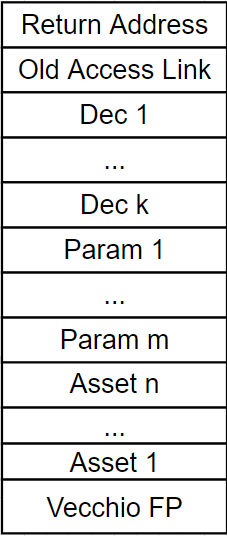
\includegraphics[width=0.9\linewidth]{RdA.png}
    \centering
\end{wrapfigure}
Durante l'esecuzione del programma a seguito delle chiamate a funzione si vengono a creare dei \emph{Record di attivazione}. La struttura del nostro record di attivazione sarà quella visibile in figura. I record di attivazione cresceranno dal basso verso l'altro, quindi il vecchio frame pointer si troverà ad indirizzi di memoria più alti del return address. Dopo aver caricato il vecchio frame pointer caricheremo prima tutti gli asset in ordine, da 1 a n. Il caricamento degli asset avviene in ordine poichè la loro dichiarazione (per mantenere coerenza con gli offset per l'accesso alle variabili nel record di attivazione) avviene al contrario. In questo modo possiamo caricare gli asset da 1 a n e conseguentemente svuotarli per mantenere la semantica di f()[a,a], in cui il primo parametro attuale sarà passato al primo formale e poi svuotato ed il secondo parametro formale riceverà un asset vuoto.  Successivamente carichiamo i parametri della funzione al contrario da m a 1 e poi il vecchio access link ed il vecchio \emph{\$ra}.
\end{document}